\newpage

% \lhead{\leftmark}
\chapter{Planning and Architecture}

\cfoot{\thepage}

\parindent=0.5in
\onehalfspacing

\section{Introduction}

The successful development of any complex software system requires thorough planning and a well-defined architecture that addresses both current requirements and future scalability needs. This chapter presents the comprehensive planning and architectural design of the TelecomOps application, a mission-critical system for managing mobile network infrastructure at Tunisie Telecom.

The planning phase encompasses detailed stakeholder analysis, requirements specification, and project organization using the Scrum methodology. The architectural design addresses the technical challenges of building a scalable, secure, and maintainable system capable of managing thousands of telecommunications sites across Tunisia's diverse geographical landscape.

Through systematic analysis of user needs, operational workflows, and technical constraints, we establish the foundation for a robust solution that enhances operational efficiency while ensuring data security and system reliability. The chapter concludes with detailed technical specifications that guide the implementation phases and ensure alignment with both business objectives and technical best practices.

\section{Stakeholder Identification and Analysis}

Stakeholder identification represents a critical foundation for understanding system requirements and designing appropriate user interfaces and access controls. Through detailed analysis of Tunisie Telecom's operational structure and telecommunications management processes, we have identified four primary stakeholder categories, each with distinct responsibilities and system interaction requirements.

\subsection{Primary Stakeholders}

\textbf{System Administrator}
\begin{itemize}
\item \textbf{Primary Responsibilities:} Complete system administration including user account management, role assignment, system configuration, and security policy enforcement
\item \textbf{Access Level:} Unrestricted access to all system functionalities including user management, system settings, and administrative dashboards
\item \textbf{Key Activities:} User provisioning, role-based access control configuration, system monitoring, backup management, and security audit coordination
\item \textbf{Usage Patterns:} Regular administrative tasks, periodic system maintenance, emergency response coordination
\end{itemize}

\textbf{Network Engineer}
\begin{itemize}
\item \textbf{Primary Responsibilities:} Technical management of network sites and equipment, configuration planning, and technical documentation maintenance
\item \textbf{Access Level:} Full access to site management, equipment configuration, technical documentation, and intervention planning
\item \textbf{Key Activities:} Site configuration management, equipment specification updates, technical intervention planning, performance analysis
\item \textbf{Usage Patterns:} Daily technical operations, planned maintenance coordination, emergency technical response
\end{itemize}

\textbf{Field Technician}
\begin{itemize}
\item \textbf{Primary Responsibilities:} On-site maintenance execution, equipment installation, fault resolution, and field data collection
\item \textbf{Access Level:} Access to assigned intervention details, site information, equipment status updates, and progress reporting
\item \textbf{Key Activities:} Intervention execution, status updates, equipment testing, documentation of completed work
\item \textbf{Usage Patterns:} Mobile access during field operations, real-time status updates, documentation completion
\end{itemize}

\textbf{Operations Manager}
\begin{itemize}
\item \textbf{Primary Responsibilities:} Strategic oversight, performance monitoring, resource allocation, and operational decision-making
\item \textbf{Access Level:} Read-only access to dashboards, reports, performance metrics, and strategic analytics
\item \textbf{Key Activities:} Performance monitoring, resource planning, strategic decision-making, stakeholder reporting
\item \textbf{Usage Patterns:} Regular dashboard review, periodic report generation, strategic planning sessions
\end{itemize}

\subsection{Stakeholder Interaction Matrix}

\begin{table}[H]
\centering
\begin{tabular}{|l|c|c|c|c|}
\hline
\textbf{System Function} & \textbf{Admin} & \textbf{Engineer} & \textbf{Technician} & \textbf{Manager} \\
\hline
User Management & Full & - & - & View \\
\hline
Site Management & Full & Full & View & View \\
\hline
Equipment Management & Full & Full & Update & View \\
\hline
Intervention Planning & Full & Full & Assigned & View \\
\hline
Alert Management & Full & Full & View & View \\
\hline
Reporting & Full & View & Limited & Full \\
\hline
System Configuration & Full & Limited & - & - \\
\hline
\end{tabular}
\caption{Stakeholder Access Control Matrix}
\label{tab:stakeholder_access}
\end{table}

\section{Requirements Specification}

Requirements specification provides the detailed foundation for system design and development, ensuring that all stakeholder needs are systematically addressed while maintaining focus on operational efficiency and technical feasibility.

\subsection{Functional Requirements Analysis}

The functional requirements have been organized into core functional domains that address the complete lifecycle of telecommunications site management operations.

\subsubsection{Authentication and Authorization Management}
\textbf{FR-001: User Authentication}
\begin{itemize}
\item Secure user login with email and password validation
\item Multi-factor authentication for administrator accounts
\item Session management with automatic timeout capabilities
\item Password reset and recovery mechanisms
\end{itemize}

\textbf{FR-002: Role-Based Access Control}
\begin{itemize}
\item Four-tier authorization hierarchy (Administrator, Engineer, Technician, Manager)
\item Granular permission management for system functions
\item Regional access control for geographical site management
\item Dynamic role assignment and modification capabilities
\end{itemize}

\subsubsection{Site Management Operations}
\textbf{FR-003: Site Information Management}
\begin{itemize}
\item Comprehensive site registration including geographical coordinates, addressing, and technical specifications
\item Support for multiple network technologies (2G, 3G, 4G, 5G installations)
\item Site status tracking (Operational, Under Maintenance, Inactive, Planned)
\item Historical data maintenance for site configuration changes
\end{itemize}

\textbf{FR-004: Geographic Information System Integration}
\begin{itemize}
\item Interactive mapping interface for site visualization
\item Geographical search and filtering capabilities
\item Distance-based analysis for resource allocation
\item Regional grouping and management hierarchies
\end{itemize}

\subsubsection{Equipment Management System}
\textbf{FR-005: Equipment Inventory Management}
\begin{itemize}
\item Detailed equipment registration with serial numbers, specifications, and installation data
\item Equipment lifecycle tracking from installation to replacement
\item Maintenance schedule management with automated reminders
\item Warranty tracking and replacement planning
\end{itemize}

\textbf{FR-006: Equipment Performance Monitoring}
\begin{itemize}
\item Real-time equipment status monitoring
\item Performance metrics collection and analysis
\item Threshold-based alert generation for equipment anomalies
\item Historical performance data analysis and trending
\end{itemize}

\subsubsection{Intervention and Maintenance Management}
\textbf{FR-007: Intervention Planning and Scheduling}
\begin{itemize}
\item Preventive maintenance scheduling based on equipment specifications and historical data
\item Emergency intervention management with priority classification
\item Resource allocation and technician assignment optimization
\item Multi-site intervention coordination for efficiency maximization
\end{itemize}

\textbf{FR-008: Field Operations Support}
\begin{itemize}
\item Mobile-optimized interface for field technician access
\item Real-time intervention status updates and progress tracking
\item Digital documentation capture including photos and technical notes
\item Parts and materials requirement tracking for inventory management
\end{itemize}

\subsubsection{Alert and Monitoring System}
\textbf{FR-009: Real-Time Alert Management}
\begin{itemize}
\item Multi-level alert classification (Critical, High, Medium, Low severity)
\item Automated alert generation based on equipment status and performance thresholds
\item Alert escalation procedures with time-based escalation rules
\item Alert acknowledgment and resolution tracking with accountability measures
\end{itemize}

\textbf{FR-010: Notification and Communication}
\begin{itemize}
\item Multi-channel notification delivery (Email, SMS, In-app notifications)
\item Role-based notification filtering and routing
\item Emergency broadcast capabilities for critical incidents
\item Communication audit trails for compliance and analysis
\end{itemize}

\subsubsection{Reporting and Analytics}
\textbf{FR-011: Operational Reporting}
\begin{itemize}
\item Standardized report templates for common operational metrics
\item Custom report generation with flexible filtering and grouping
\item Automated report scheduling and distribution
\item Data export capabilities in multiple formats (PDF, Excel, CSV)
\end{itemize}

\textbf{FR-012: Performance Analytics}
\begin{itemize}
\item Key Performance Indicator (KPI) dashboards for operational oversight
\item Trend analysis for proactive maintenance planning
\item Resource utilization analytics for optimization opportunities
\item Comparative analysis across regions, sites, and equipment types
\end{itemize}

\subsection{Non-Functional Requirements}

Non-functional requirements ensure that the system meets operational, performance, and quality standards necessary for mission-critical telecommunications infrastructure management.

\subsubsection{Performance Requirements}
\textbf{NFR-001: Response Time Performance}
\begin{itemize}
\item Web page load times under 3 seconds for standard operations
\item API response times under 500 milliseconds for data queries
\item Real-time update propagation within 2 seconds across all connected clients
\item Dashboard refresh intervals configurable from 30 seconds to 5 minutes
\end{itemize}

\textbf{NFR-002: Scalability and Capacity}
\begin{itemize}
\item Support for minimum 5,000 network sites with growth capacity to 10,000
\item Concurrent user support for up to 200 simultaneous active sessions
\item Data retention capabilities for minimum 5 years of historical records
\item Horizontal scaling capabilities for increased load management
\end{itemize}

\subsubsection{Security and Compliance}
\textbf{NFR-003: Data Security}
\begin{itemize}
\item End-to-end encryption for all data transmission using TLS 1.3
\item Database encryption at rest with industry-standard algorithms
\item Role-based data access control with row-level security implementation
\item Security audit logging for all user actions and system changes
\end{itemize}

\textbf{NFR-004: Authentication Security}
\begin{itemize}
\item Multi-factor authentication for administrative accounts
\item Password complexity requirements with regular rotation policies
\item Session management with automatic timeout and concurrent session control
\item Failed login attempt monitoring with account lockout mechanisms
\end{itemize}

\subsubsection{Reliability and Availability}
\textbf{NFR-005: System Availability}
\begin{itemize}
\item 99.5\% uptime availability target with planned maintenance windows
\item Automated backup procedures with point-in-time recovery capabilities
\item Disaster recovery procedures with maximum 4-hour recovery time objective
\item Redundancy implementation for critical system components
\end{itemize}

\subsubsection{Usability and Accessibility}
\textbf{NFR-006: User Experience}
\begin{itemize}
\item Responsive design supporting desktop, tablet, and mobile devices
\item Multi-language support (French, Arabic, English) for user interfaces
\item Accessibility compliance with WCAG 2.1 guidelines
\item Intuitive navigation with maximum 3-click access to primary functions
\end{itemize}

\section{Product Backlog and User Stories}

The product backlog represents a prioritized list of features and functionality organized as user stories that capture specific user needs and system capabilities. Each user story follows the standard format "As a [user type], I want [functionality] so that [benefit]" to ensure clear understanding of user requirements and expected outcomes.

\subsection{High Priority User Stories}

\begin{longtable}{|c|p{3.5cm}|p{7.5cm}|c|}
\caption{Product Backlog - High Priority Features} \\
\hline
\textbf{ID} & \textbf{Feature Category} & \textbf{User Story} & \textbf{Priority} \\
\hline
\endfirsthead
\hline
\textbf{ID} & \textbf{Feature Category} & \textbf{User Story} & \textbf{Priority} \\
\hline
\endhead
US-001 & Authentication System & As any user, I want to securely log into the system using my credentials so that I can access authorized functionalities based on my role & High \\
\hline
US-002 & User Profile Management & As any user, I want to manage my profile information and change my password so that I can maintain account security and current information & High \\
\hline
US-003 & Site Management & As an Administrator or Network Engineer, I want to create, modify, and delete site records so that I can maintain accurate site information for network operations & High \\
\hline
US-004 & Site Information Access & As a Field Technician or Manager, I want to view detailed site information so that I can understand site specifications and current status & High \\
\hline
US-005 & Equipment Management & As an Administrator or Network Engineer, I want to manage equipment inventory including specifications, installation dates, and maintenance schedules so that I can track equipment lifecycle effectively & High \\
\hline
US-006 & Equipment Status Monitoring & As any user, I want to view current equipment status and performance metrics so that I can assess equipment health and identify potential issues & High \\
\hline
US-007 & Intervention Planning & As an Administrator or Network Engineer, I want to create and schedule maintenance interventions so that I can ensure proactive equipment maintenance and minimize downtime & High \\
\hline
US-008 & Technician Assignment & As an Administrator or Network Engineer, I want to assign interventions to specific field technicians so that I can optimize resource allocation and ensure accountability & High \\
\hline
US-009 & Intervention Tracking & As a Field Technician, I want to update intervention status and document completed work so that I can provide accurate progress information to management & High \\
\hline
US-010 & Alert Generation & As the system, I want to automatically generate alerts based on equipment status and performance thresholds so that users can respond quickly to potential issues & High \\
\hline
\end{longtable}

\subsection{Medium Priority User Stories}

\begin{longtable}{|c|p{3.5cm}|p{7.5cm}|c|}
\caption{Product Backlog - Medium Priority Features} \\
\hline
\textbf{ID} & \textbf{Feature Category} & \textbf{User Story} & \textbf{Priority} \\
\hline
\endfirsthead
\hline
\textbf{ID} & \textbf{Feature Category} & \textbf{User Story} & \textbf{Priority} \\
\hline
\endhead
US-011 & Alert Management & As an Administrator or Network Engineer, I want to manage alert configurations and resolution procedures so that I can optimize alert effectiveness and reduce false positives & Medium \\
\hline
US-012 & Geographic Mapping & As any user, I want to view sites on an interactive map so that I can visualize geographical distribution and plan field operations efficiently & Medium \\
\hline
US-013 & Performance Dashboards & As a Manager, I want to view operational dashboards with key performance indicators so that I can monitor overall system performance and make informed decisions & Medium \\
\hline
US-014 & Report Generation & As an Administrator or Manager, I want to generate standardized reports on site performance and maintenance activities so that I can analyze trends and prepare management summaries & Medium \\
\hline
US-015 & Data Export & As any authorized user, I want to export data in various formats (PDF, Excel, CSV) so that I can use information in external systems and presentations & Medium \\
\hline
US-016 & Equipment Specifications & As an Administrator, I want to manage equipment type specifications and maintenance requirements so that I can standardize equipment management procedures & Medium \\
\hline
US-017 & Maintenance Cost Tracking & As an Administrator or Manager, I want to track maintenance costs and resource utilization so that I can optimize operational budgets and resource allocation & Medium \\
\hline
US-018 & Historical Data Analysis & As a Network Engineer or Manager, I want to analyze historical performance and maintenance data so that I can identify trends and improve preventive maintenance strategies & Medium \\
\hline
\end{longtable}

\subsection{Low Priority User Stories}

\begin{longtable}{|c|p{3.5cm}|p{7.5cm}|c|}
\caption{Product Backlog - Low Priority Features} \\
\hline
\textbf{ID} & \textbf{Feature Category} & \textbf{User Story} & \textbf{Priority} \\
\hline
\endfirsthead
\hline
\textbf{ID} & \textbf{Feature Category} & \textbf{User Story} & \textbf{Priority} \\
\hline
\endhead
US-019 & Advanced Analytics & As a Manager, I want to access predictive analytics for equipment failure prediction so that I can implement proactive replacement strategies & Low \\
\hline
US-020 & Mobile Application & As a Field Technician, I want to access system functionality through a dedicated mobile application so that I can work efficiently during field operations & Low \\
\hline
US-021 & Integration APIs & As a System Administrator, I want to integrate with external monitoring systems through APIs so that I can consolidate network management operations & Low \\
\hline
US-022 & Automated Notifications & As any user, I want to configure automated notifications for specific events so that I can receive timely information about relevant system changes & Low \\
\hline
US-023 & Audit Trail Management & As an Administrator, I want to access comprehensive audit trails for all system changes so that I can ensure compliance and security oversight & Low \\
\hline
\end{longtable}

\section{Sprint Planning and Development Methodology}

The TelecomOps project adopts the Scrum framework for agile development, organizing work into six distinct sprints that progressively build system capabilities while ensuring continuous stakeholder feedback and iterative improvement.

\subsection{Sprint Organization and Timeline}

\begin{table}[H]
\centering
\begin{tabular}{|c|p{2.5cm}|p{8cm}|c|}
\hline
\textbf{Sprint} & \textbf{Duration} & \textbf{Primary Deliverables} & \textbf{User Stories} \\
\hline
Sprint 1 & Weeks 1-2 & Authentication System, User Management, Role-based Access Control, Profile Management & US-001, US-002 \\
\hline
Sprint 2 & Weeks 3-4 & Site Management, Geographic Mapping, Site Status Monitoring, Network Technology Support & US-003, US-004, US-012 \\
\hline
Sprint 3 & Weeks 5-6 & Equipment Management, Equipment Tracking, Maintenance Schedules, Equipment Specifications & US-005, US-006, US-016 \\
\hline
Sprint 4 & Weeks 7-8 & Intervention Management, Technician Assignment, Status Tracking, Field Operations Support & US-007, US-008, US-009 \\
\hline
Sprint 5 & Weeks 9-10 & Alert System, Real-time Monitoring, Severity Classification, Alert Management & US-010, US-011 \\
\hline
Sprint 6 & Weeks 11-12 & Reporting \& Analytics, Performance Dashboards, Data Export, System Optimization & US-013, US-014, US-015, US-017 \\
\hline
\end{tabular}
\caption{Sprint Planning Overview}
\label{tab:sprint_planning}
\end{table}

\subsection{Sprint Objectives and Success Criteria}

\subsubsection{Sprint 1: Foundation (Authentication \& User Management)}
\textbf{Primary Objectives:}
\begin{itemize}
\item Establish secure authentication framework using Supabase Auth
\item Implement role-based access control with four user types
\item Create user profile management capabilities
\item Set up project infrastructure and development environment
\end{itemize}

\textbf{Success Criteria:}
\begin{itemize}
\item Users can securely log in and access role-appropriate functionalities
\item Administrator can manage user accounts and role assignments
\item Password reset and profile update functionalities operational
\item Development environment fully configured with CI/CD pipeline
\end{itemize}

\subsubsection{Sprint 2: Site Management}
\textbf{Primary Objectives:}
\begin{itemize}
\item Develop comprehensive site management interface
\item Implement geographic mapping with interactive capabilities
\item Create site status monitoring and reporting features
\item Support multiple network technology classifications
\end{itemize}

\textbf{Success Criteria:}
\begin{itemize}
\item Sites can be created, modified, and deleted by authorized users
\item Geographic map displays all sites with accurate positioning
\item Site status updates reflect in real-time across user sessions
\item Network technology filtering and search capabilities functional
\end{itemize}

\subsubsection{Sprint 3: Equipment Management}
\textbf{Primary Objectives:}
\begin{itemize}
\item Build equipment inventory management system
\item Implement equipment lifecycle tracking capabilities
\item Create maintenance scheduling and reminder systems
\item Develop equipment specification management interface
\end{itemize}

\textbf{Success Criteria:}
\begin{itemize}
\item Equipment records include complete specification and maintenance data
\item Maintenance schedules generate automated reminders
\item Equipment status monitoring reflects current operational state
\item Equipment search and filtering capabilities functional across all sites
\end{itemize}

\subsubsection{Sprint 4: Intervention Management}
\textbf{Primary Objectives:}
\begin{itemize}
\item Develop intervention planning and scheduling system
\item Implement technician assignment and resource allocation
\item Create field operations support interface for mobile access
\item Build intervention tracking and progress monitoring capabilities
\end{itemize}

\textbf{Success Criteria:}
\begin{itemize}
\item Interventions can be scheduled and assigned to specific technicians
\item Field technicians can update intervention status in real-time
\item Resource allocation optimizes technician assignments based on location and expertise
\item Intervention history provides complete audit trail for maintenance activities
\end{itemize}

\subsubsection{Sprint 5: Alert System}
\textbf{Primary Objectives:}
\begin{itemize}
\item Implement real-time alert generation and management
\item Create severity-based alert classification system
\item Develop alert escalation and notification procedures
\item Build alert acknowledgment and resolution tracking
\end{itemize}

\textbf{Success Criteria:}
\begin{itemize}
\item Alerts generate automatically based on equipment status thresholds
\item Alert severity determines notification routing and escalation procedures
\item Users receive appropriate notifications based on role and responsibility
\item Alert resolution tracking provides accountability and performance metrics
\end{itemize}

\subsubsection{Sprint 6: Reporting \& Analytics}
\textbf{Primary Objectives:}
\begin{itemize}
\item Develop comprehensive reporting capabilities with standardized templates
\item Create performance analytics dashboards for operational oversight
\item Implement data export functionality in multiple formats
\item Build cost tracking and resource utilization analytics
\end{itemize}

\textbf{Success Criteria:}
\begin{itemize}
\item Standardized reports generate automatically with accurate data
\item Dashboard visualizations provide actionable insights for decision-making
\item Data export functionality supports multiple formats and user requirements
\item Cost and resource analytics enable optimization of operational efficiency
\end{itemize}

\section{Use Case Analysis}

Use case analysis provides detailed examination of system interactions from the user perspective, ensuring that all functional requirements are captured and properly addressed in the system design.

\subsection{Global Use Case Overview}

\begin{figure}[H]
    \centering
    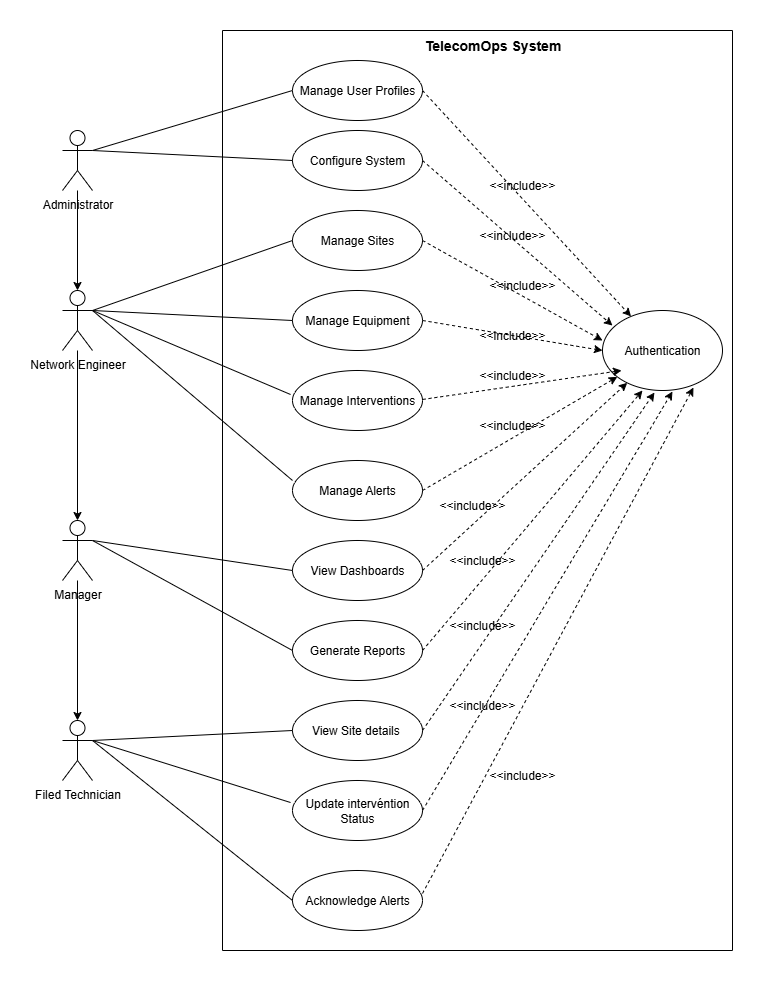
\includegraphics[width=0.95\linewidth]{img/chap_02/TelecomOps_UseCase_Diagram.png}
    \caption{TelecomOps Global Use Case Diagram}
    \label{fig:use_case_global}
\end{figure}

The global use case diagram illustrates the comprehensive interaction patterns between different stakeholder types and system functionalities, providing a visual representation of system scope and user accessibility patterns.

\subsection{Detailed Use Case Specifications}

\subsubsection{Use Case: Site Management}
\textbf{Use Case ID:} UC-001 \\
\textbf{Primary Actors:} Administrator, Network Engineer \\
\textbf{Secondary Actors:} Field Technician (view only), Manager (view only) \\
\textbf{Preconditions:} User authenticated with appropriate role permissions \\

\textbf{Main Success Scenario:}
\begin{enumerate}
\item User navigates to site management interface
\item System displays current site inventory with filtering and search capabilities
\item User selects site creation, modification, or deletion action
\item System presents appropriate data entry or confirmation interface
\item User completes required information and submits changes
\item System validates data and updates site records
\item System confirms successful operation and updates displays
\end{enumerate}

\textbf{Alternative Flows:}
\begin{itemize}
\item Data validation failures result in error messages and correction opportunities
\item Unauthorized access attempts redirect to appropriate access level interface
\item Site deletion requires confirmation and checks for dependent records
\end{itemize}

\subsubsection{Use Case: Equipment Monitoring}
\textbf{Use Case ID:} UC-002 \\
\textbf{Primary Actors:} All user types \\
\textbf{Preconditions:} User authenticated with site access permissions \\

\textbf{Main Success Scenario:}
\begin{enumerate}
\item User selects specific site for equipment monitoring
\item System retrieves and displays current equipment inventory and status
\item User accesses detailed equipment information including performance metrics
\item System provides real-time status updates and historical performance data
\item User can filter and search equipment based on various criteria
\item System enables appropriate actions based on user role permissions
\end{enumerate}

\subsubsection{Use Case: Intervention Management}
\textbf{Use Case ID:} UC-003 \\
\textbf{Primary Actors:} Administrator, Network Engineer, Field Technician \\
\textbf{Preconditions:} User authenticated with intervention access permissions \\

\textbf{Main Success Scenario:}
\begin{enumerate}
\item Authorized user creates new intervention or accesses existing interventions
\item System presents intervention details including site, equipment, and scheduling information
\item User updates intervention status, assigns resources, or documents progress
\item System validates changes and updates intervention records
\item System generates notifications to relevant stakeholders
\item System maintains audit trail of all intervention activities
\end{enumerate}

\section{System Architecture}

The TelecomOps system architecture implements a modern, scalable design that addresses the complex requirements of telecommunications infrastructure management while ensuring security, performance, and maintainability.

\subsection{Architectural Overview}

The system follows a three-tier architecture pattern that provides clear separation of concerns and enables independent scaling of different system components.

\begin{figure}[H]
    \centering
    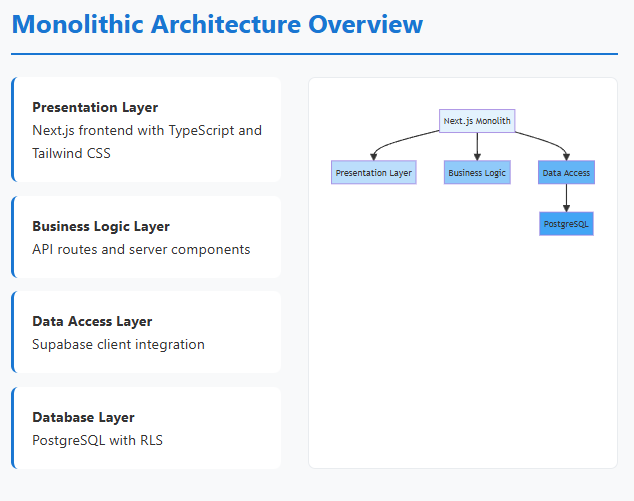
\includegraphics[width=0.9\linewidth]{img/chap_02/architecture_overview.png}
    \caption{TelecomOps Three-Tier Architecture}
    \label{fig:architecture_overview}
\end{figure}

\subsubsection{Presentation Layer}
The presentation layer implements a responsive, progressive web application using modern frontend technologies:

\textbf{Technology Stack:}
\begin{itemize}
\item \textbf{Next.js 14:} React-based framework providing server-side rendering, automatic code splitting, and optimized performance
\item \textbf{TypeScript:} Type-safe JavaScript superset ensuring code reliability and enhanced developer experience
\item \textbf{Tailwind CSS:} Utility-first CSS framework enabling rapid, consistent interface development
\item \textbf{Shadcn/UI:} High-quality, accessible component library built on Radix UI primitives
\end{itemize}

\textbf{Key Capabilities:}
\begin{itemize}
\item Responsive design supporting desktop, tablet, and mobile devices
\item Progressive Web App features including offline capabilities and push notifications
\item Server-side rendering for improved performance and SEO optimization
\item Real-time data updates through WebSocket connections
\end{itemize}

\subsubsection{Application Layer}
The application layer provides comprehensive backend services through the Supabase platform:

\textbf{Core Services:}
\begin{itemize}
\item \textbf{Authentication Service:} Secure user authentication with JWT tokens and role-based access control
\item \textbf{Database API:} Auto-generated RESTful APIs based on PostgreSQL database schema
\item \textbf{Real-time Engine:} WebSocket-based real-time subscriptions for live data updates
\item \textbf{Storage Service:} File storage and management for documentation and media assets
\end{itemize}

\subsubsection{Data Layer}
The data layer implements a robust PostgreSQL database with advanced security and performance features:

\textbf{Database Features:}
\begin{itemize}
\item \textbf{Row Level Security (RLS):} Fine-grained access control at the database level
\item \textbf{JSONB Support:} Flexible storage for complex configuration and specification data
\item \textbf{Full-text Search:} Advanced search capabilities across multiple data types
\item \textbf{Automated Backups:} Point-in-time recovery with configurable retention policies
\end{itemize}

\subsection{Database Design and Schema}

The database schema implements a normalized relational design optimized for telecommunications operations while maintaining flexibility for future enhancements.

\begin{figure}[H]
    \centering
    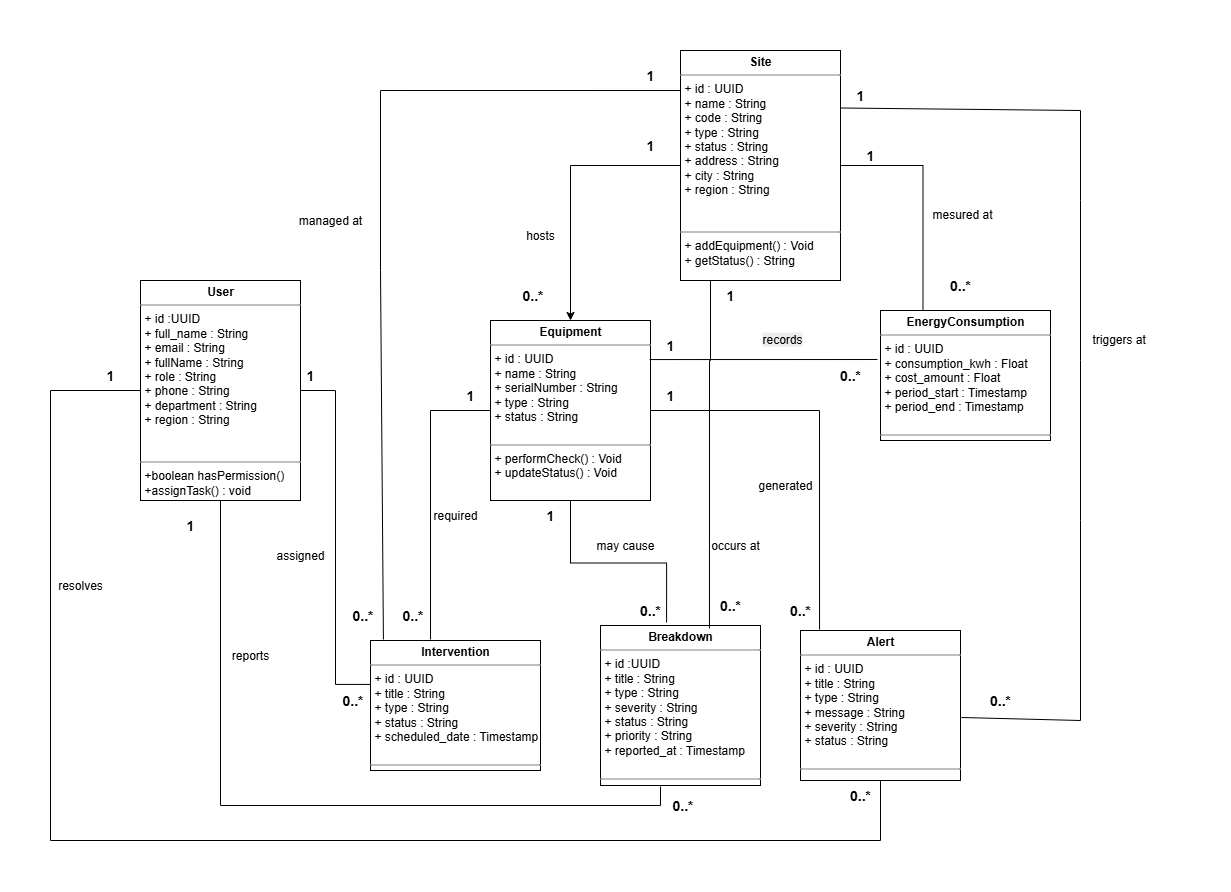
\includegraphics[width=0.85\linewidth]{img/chap_02/database_er_diagram.png}
    \caption{TelecomOps Database Entity-Relationship Diagram}
    \label{fig:database_er_diagram}
\end{figure}

\subsubsection{Core Entity Specifications}

\textbf{Profiles Entity}
\begin{itemize}
\item Stores user account information linked to Supabase authentication
\item Includes role assignment and regional access control
\item Maintains user preferences and customization settings
\item Supports audit trail tracking for user actions
\end{itemize}

\textbf{Sites Entity}
\begin{itemize}
\item Comprehensive site information including geographical coordinates
\item Network technology support (2G, 3G, 4G, 5G) with configuration details
\item Operational status tracking with timestamp information
\item Relationship management for equipment and intervention associations
\end{itemize}

\textbf{Equipment Entity}
\begin{itemize}
\item Detailed equipment specifications using JSONB for flexibility
\item Serial number tracking with warranty and lifecycle information
\item Performance metrics storage with historical data retention
\item Maintenance schedule integration with automated reminder generation
\end{itemize}

\textbf{Interventions Entity}
\begin{itemize}
\item Comprehensive intervention tracking from planning to completion
\item Technician assignment with skill and availability matching
\item Documentation storage including photos and technical notes
\item Cost tracking and resource utilization analytics
\end{itemize}

\textbf{Alerts Entity}
\begin{itemize}
\item Multi-level severity classification with escalation rules
\item Automatic generation based on equipment status and performance thresholds
\item Acknowledgment and resolution tracking with accountability measures
\item Integration with notification systems for multi-channel delivery
\end{itemize}

\subsection{Security Architecture}

Security implementation follows defense-in-depth principles with multiple layers of protection ensuring data confidentiality, integrity, and availability.

\begin{figure}[H]
    \centering
    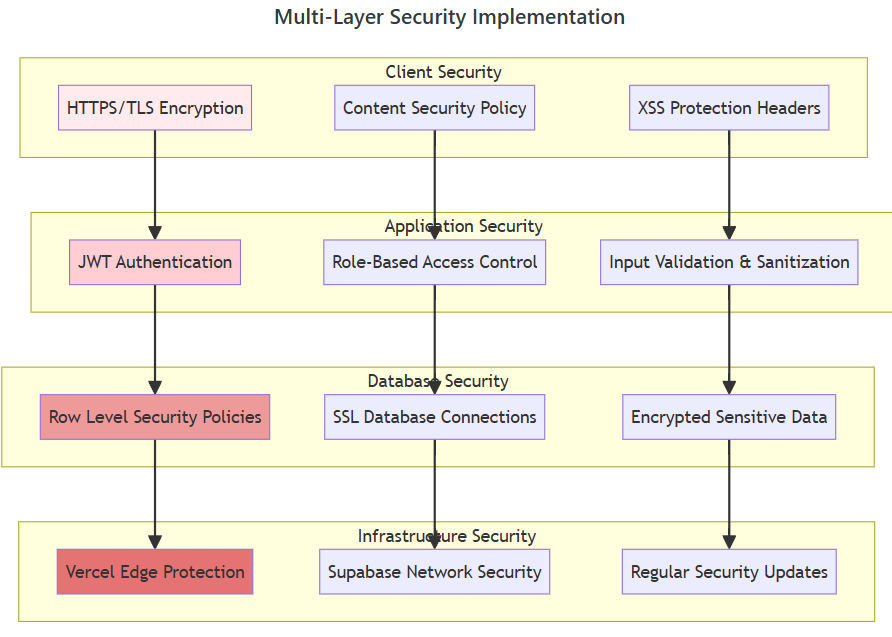
\includegraphics[width=1\linewidth]{img/chap_02/security_architecture.png}
    \caption{Multi-Layer Security Architecture}
    \label{fig:security_architecture}
\end{figure}

\subsubsection{Transport Security}
\begin{itemize}
\item TLS 1.3 encryption for all client-server communication
\item Certificate management through automated renewal processes
\item HTTP Strict Transport Security (HSTS) implementation
\item Content Security Policy (CSP) headers for XSS protection
\end{itemize}

\subsubsection{Application Security}
\begin{itemize}
\item JWT-based authentication with configurable token expiration
\item Role-based access control with granular permission management
\item API rate limiting to prevent abuse and ensure availability
\item Input validation and sanitization for all user-provided data
\end{itemize}

\subsubsection{Database Security}
\begin{itemize}
\item Row Level Security policies enforcing data access controls
\item Encryption at rest for all sensitive data storage
\item Connection encryption using SSL/TLS protocols
\item Comprehensive audit logging for all database operations
\end{itemize}

\subsubsection{Infrastructure Security}
\begin{itemize}
\item Web Application Firewall (WAF) protection against common threats
\item DDoS mitigation through cloud-based protection services
\item Network isolation and secure deployment practices
\item Automated security monitoring and incident response capabilities
\end{itemize}

\section{Technology Stack Justification}

The selection of technologies for the TelecomOps platform prioritizes reliability, scalability, security, and development efficiency while ensuring alignment with modern software engineering best practices.

\subsection{Frontend Technology Selection}

\subsubsection{Next.js Framework}
\textbf{Selection Rationale:}
\begin{itemize}
\item \textbf{Performance Optimization:} Built-in server-side rendering and automatic code splitting reduce initial load times and improve user experience
\item \textbf{Developer Experience:} Comprehensive tooling, hot reloading, and TypeScript integration accelerate development cycles
\item \textbf{Production Readiness:} Automatic optimizations, image optimization, and performance monitoring capabilities
\item \textbf{Ecosystem Compatibility:} Seamless integration with React ecosystem and modern development tools
\end{itemize}

\subsubsection{TypeScript Implementation}
\textbf{Selection Rationale:}
\begin{itemize}
\item \textbf{Type Safety:} Compile-time error detection reduces runtime errors and improves code reliability
\item \textbf{Developer Productivity:} Enhanced IDE support with autocompletion and refactoring capabilities
\item \textbf{Maintainability:} Self-documenting code through type definitions and interfaces
\item \textbf{Team Collaboration:} Clear contracts between components facilitate team development
\end{itemize}

\subsubsection{Tailwind CSS Framework}
\textbf{Selection Rationale:}
\begin{itemize}
\item \textbf{Development Speed:} Utility-first approach enables rapid prototyping and interface development
\item \textbf{Consistency:} Predefined design tokens ensure consistent spacing, colors, and typography
\item \textbf{Customization:} Flexible configuration supports brand-specific design requirements
\item \textbf{Performance:} Purging unused styles results in minimal production bundle sizes
\end{itemize}

\subsection{Backend Technology Selection}

\subsubsection{Supabase Platform}
\textbf{Selection Rationale:}
\begin{itemize}
\item \textbf{Development Acceleration:} Backend-as-a-Service approach reduces infrastructure setup and maintenance overhead
\item \textbf{PostgreSQL Foundation:} Mature, reliable database with advanced features including JSONB support and full-text search
\item \textbf{Real-time Capabilities:} Built-in WebSocket support enables live data updates without additional infrastructure
\item \textbf{Security Implementation:} Row Level Security and authentication services provide enterprise-grade security
\item \textbf{Scalability:} Managed infrastructure with automatic scaling and performance optimization
\end{itemize}

\subsubsection{PostgreSQL Database}
\textbf{Selection Rationale:}
\begin{itemize}
\item \textbf{Data Integrity:} ACID compliance ensures data consistency in mission-critical telecommunications operations
\item \textbf{Advanced Features:} JSONB support, full-text search, and geographic data types address complex requirements
\item \textbf{Performance:} Mature query optimizer and indexing capabilities support high-performance operations
\item \textbf{Extensibility:} Rich ecosystem of extensions and functions support specialized telecommunications requirements
\end{itemize}

\subsection{Deployment and Infrastructure}

\subsubsection{Vercel Platform}
\textbf{Selection Rationale:}
\begin{itemize}
\item \textbf{Next.js Optimization:} Purpose-built platform for Next.js applications with automatic optimizations
\item \textbf{Global Distribution:} Edge network ensures optimal performance for users across different geographical locations
\item \textbf{Automatic Deployments:} Git-based deployment workflow with preview environments for testing
\item \textbf{Monitoring Integration:} Built-in analytics and performance monitoring capabilities
\end{itemize}

\subsubsection{Supabase Cloud}
\textbf{Selection Rationale:}
\begin{itemize}
\item \textbf{Managed Services:} Automated backups, security updates, and infrastructure management
\item \textbf{Global Availability:} Multi-region deployment options for improved performance and disaster recovery
\item \textbf{Compliance:} SOC 2 Type II certification and GDPR compliance for regulatory requirements
\item \textbf{Cost Effectiveness:} Predictable pricing model with scaling based on actual usage
\end{itemize}

\section{Deployment Architecture}

The deployment architecture ensures high availability, optimal performance, and seamless scaling to meet the demands of telecommunications infrastructure management.

\begin{figure}[H]
    \centering
    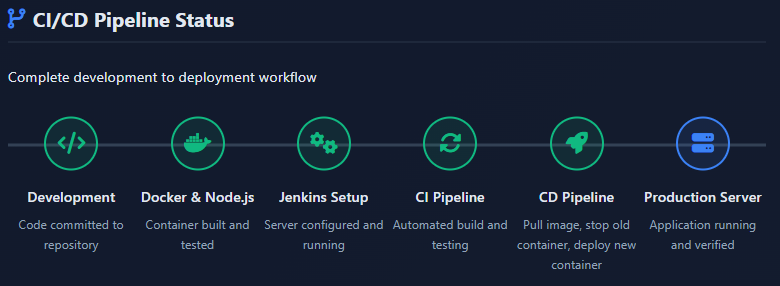
\includegraphics[width=0.85\linewidth]{img/chap_02/deployment_architecture.png}
    \caption{Cloud Deployment Architecture}
    \label{fig:deployment_architecture}
\end{figure}

\subsection{Frontend Deployment Strategy}

\subsubsection{Vercel Edge Network}
\begin{itemize}
\item Global CDN distribution with edge locations across multiple continents
\item Automatic HTTPS with custom domain support and SSL certificate management
\item Server-side rendering capabilities with edge computing for optimal performance
\item Automatic image optimization and responsive image delivery
\end{itemize}

\subsubsection{Performance Optimization}
\begin{itemize}
\item Automatic code splitting and lazy loading for reduced initial bundle sizes
\item Static asset optimization with compression and caching strategies
\item Progressive Web App capabilities including service worker implementation
\item Performance monitoring with Core Web Vitals tracking and optimization suggestions
\end{itemize}

\subsection{Backend Deployment Strategy}

\subsubsection{Supabase Infrastructure}
\begin{itemize}
\item Managed PostgreSQL instances with automatic scaling and performance optimization
\item Multi-region deployment options for improved latency and disaster recovery
\item Automated backup procedures with point-in-time recovery capabilities
\item Built-in monitoring and logging with custom alerting configurations
\end{itemize}

\subsubsection{API Gateway and Load Balancing}
\begin{itemize}
\item Automatic load balancing across multiple database replicas
\item Connection pooling for optimal database resource utilization
\item Rate limiting and DDoS protection at the infrastructure level
\item Health checking and automatic failover mechanisms
\end{itemize}

\subsection{Monitoring and Observability}

\subsubsection{Application Performance Monitoring}
\begin{itemize}
\item Real-time performance metrics collection and analysis
\item Error tracking and automated alerting for critical issues
\item User experience monitoring with Core Web Vitals and user journey analysis
\item Custom dashboard creation for operational metrics and KPIs
\end{itemize}

\subsubsection{Infrastructure Monitoring}
\begin{itemize}
\item Database performance monitoring with query analysis and optimization suggestions
\item Resource utilization tracking for capacity planning and cost optimization
\item Security monitoring with automated threat detection and response
\item Audit logging and compliance reporting for regulatory requirements
\end{itemize}

\section*{Conclusion}

This chapter has established a comprehensive planning and architectural foundation for the TelecomOps project, providing detailed specifications that ensure systematic development of a robust telecommunications infrastructure management solution. Through thorough stakeholder analysis, we have identified four distinct user roles with specific operational requirements and access patterns that drive the system's role-based security architecture.

The requirements specification encompasses both functional capabilities essential for telecommunications operations and non-functional requirements that ensure system reliability, security, and performance under operational conditions. The product backlog, organized into 23 prioritized user stories, provides a clear development roadmap that addresses core telecommunications management needs while enabling future enhancement opportunities.

The six-sprint development approach, implementing Scrum methodology, ensures iterative delivery of value while maintaining stakeholder engagement and enabling continuous refinement of system capabilities. Each sprint focuses on specific functional domains, building progressively from foundational authentication and user management through advanced analytics and reporting capabilities.

The technical architecture, combining Next.js frontend technology with Supabase backend services, provides a modern, scalable foundation that addresses the complex requirements of mobile network infrastructure management. The three-tier architecture ensures clear separation of concerns while enabling independent scaling and maintenance of different system components.

The comprehensive security architecture implements defense-in-depth principles with multiple layers of protection, ensuring that sensitive telecommunications infrastructure data remains secure while enabling appropriate access for operational teams. The integration of Row Level Security with role-based access control provides granular data protection that aligns with organizational security policies.

Technology selection prioritizes proven, mature solutions that balance development efficiency with operational reliability. The chosen stack enables rapid development while providing enterprise-grade capabilities for security, performance, and scalability. The deployment architecture leverages cloud-native approaches to ensure high availability and optimal performance for users across Tunisia's geographical regions.

With this comprehensive planning and architectural foundation established, the project is well-positioned for systematic implementation that addresses the operational needs of Tunisie Telecom's mobile network infrastructure management while providing a scalable platform for future technological evolution and business growth.